% Filename: lista11.tex
% 
% This code is part of 'Solutions for MT402, Matrizes'
% 
% Description: This file corresponds to the solutions of homework sheet 11.
% 
% Created: 12.06.12 03:01:45 PM
% Last Change: 29.06.12 05:38:52 PM
% 
% Authors:
% - Raniere Silva (2012): initial version
%
% Copyright (c) 2012 Raniere Silva <r.gaia.cs@gmail.com>
% 
% This work is licensed under the Creative Commons Attribution-ShareAlike 3.0 Unported License. To view a copy of this license, visit http://creativecommons.org/licenses/by-sa/3.0/ or send a letter to Creative Commons, 444 Castro Street, Suite 900, Mountain View, California, 94041, USA.
%
% This work is distributed in the hope that it will be useful, but WITHOUT ANY WARRANTY; without even the implied warranty of MERCHANTABILITY or FITNESS FOR A PARTICULAR PURPOSE.
%
\documentclass[a4paper,12pt, leqno, answers]{exam}
% Customiza\c{c}\~{a}o da classe exam
\newcommand{\mycheader}{Lista 11 - Decomposi\c{c}\~{a}o SVD}
\header{MT402}{\mycheader}{\thepage/\numpages}
\headrule
\footer{Dispon\'{i}vel em \\\url{https://github.com/r-gaia-cs/solucoes_lista_matrizes}
}{}{Reportar erros para \\\href{mailto:r.gaia.cs@gmail.com}{r.gaia.cs@gmail.com}
}
\footrule 
\pagestyle{headandfoot}
\renewcommand{\solutiontitle}{\noindent\textbf{Solu\c{c}\~{a}o:}\enspace}
\SolutionEmphasis{\slshape}
\unframedsolutions
\pointname{}

% Filename: paper_size.tex
% 
% This code is part of 'Solutions for MT402, Matrizes'
% 
% Description: This file corresponds to the paper size output.
% 
% Created: 08.05.12 09:46:55 PM
% Last Change: 04.06.12 10:42:01 PM
% 
% Authors:
% - Raniere Silva (2012): initial version
% 
% Copyright (c) 2012 Raniere Silva <r.gaia.cs@gmail.com>
% 
% This work is licensed under the Creative Commons Attribution-ShareAlike 3.0 Unported License. To view a copy of this license, visit http://creativecommons.org/licenses/by-sa/3.0/ or send a letter to Creative Commons, 444 Castro Street, Suite 900, Mountain View, California, 94041, USA.
%
% This work is distributed in the hope that it will be useful, but WITHOUT ANY WARRANTY; without even the implied warranty of MERCHANTABILITY or FITNESS FOR A PARTICULAR PURPOSE.
%
% Para impress\~{a}o
\usepackage[top=3cm, bottom=3cm, left=2cm, right=2cm]{geometry}

% Para ereaders (Kindle, Nook, Kobo, ...) and tablets (iPad, GalaxyTab, ...)
% \usepackage[papersize={180mm,240mm},margin=2mm]{geometry}
% \sloppy


% Pacotes
\usepackage[utf8]{inputenc}
\usepackage[T1]{fontenc}
\usepackage[brazil]{babel}
\usepackage{amsmath}
\usepackage{amsfonts}
\usepackage{amssymb}
\usepackage{hyperref}
\usepackage{graphicx}

% Customiza\c{c}\~{a}o do pacote amsmath
\allowdisplaybreaks[4]

% Novos ambientes
% \newenvironment{fwsolution}{\begin{EnvFullwidth}\begin{TheSolution}}{\end{TheSolution}\end{EnvFullwidth}}

% Novos comandos
% \newcommand{\mdot}{\text{\LARGE $\boldsymbol{\cdot}$}}
\newcommand{\mdot}{\bullet}

\begin{document}
%cover
\thispagestyle{empty}
% Filename: cover.tex
% 
% This code is part of 'Solutions for MT402, Matrizes'
% 
% Description: This file corresponds to the cover.
% 
% Created: 30.05.12 04:40:25 PM
% Last Change: 14.07.12 10:49:33 AM
% 
% Authors:
% - Raniere Silva (2012): initial version
% 
% Copyright (c) 2012 Raniere Silva <r.gaia.cs@gmail.com>
% 
% This work is licensed under the Creative Commons Attribution-ShareAlike 3.0 Unported License. To view a copy of this license, visit http://creativecommons.org/licenses/by-sa/3.0/ or send a letter to Creative Commons, 444 Castro Street, Suite 900, Mountain View, California, 94041, USA.
%
% This work is distributed in the hope that it will be useful, but WITHOUT ANY WARRANTY; without even the implied warranty of MERCHANTABILITY or FITNESS FOR A PARTICULAR PURPOSE.
%
\begin{center}
    \LARGE{Solu\c{c}\~{o}es para MT402, Matrizes}
    
    \Large{\mycheader}
\end{center}
\vspace{.5\textheight}

\begin{tabular}{|p{.9\textwidth}|}
\hline
Este trabalho foi licenciado com a Licen\c{c}a Creative Commons Atribui\c{c}\~{a}o - CompartilhaIgual 3.0 N\~{a}o Adaptada. Para ver uma c\'{o}pia desta licen\c{c}a, visite \url{http://creativecommons.org/licenses/by-sa/3.0/} ou envie um pedido por carta para Creative Commons, 444 Castro Street, Suite 900, Mountain View, California, 94041, USA.
\begin{center}

\includegraphics[scale=1]{cc-by-sa.png}
\end{center}
Este trabalho encontra-se dispon\'{i}vel em \url{https://github.com/r-gaia-cs/solucoes_lista_matrizes}
 e atualmente precisa de um mantenedor, se tiver interessse entre em contato com Raniere Silva (\href{mailto:r.gaia.cs@gmail.com}{r.gaia.cs@gmail.com}
).

Este trabalho \'{e} distribuido na esperança que possa ser \'{u}til, mas SEM NENHUMA GARANTIA; sem uma garantia implicita de ADEQUA\c{C}\~{A}O a qualquer MERCADO ou APLICA\c{C}\~{A}O EM PARTICULAR.
\\ \hline
\end{tabular}



\newpage
\setcounter{page}{1}
Nos exerc\'{i}cios abaixo, considere a matriz $A : m \times n$ e sua decomposi\c{c}\~{a}o SVD dada por $A = U D V^t$, onde $U : m \times m$ e $V : n \times n$ s\~{a}o matrizes ortogonais e $D : m \times n$ \'{e} tal que $d_{ij} = 0$ para $i \neq j$ e $d_{ii} = \sigma_i$, $i = 1, 2, \ldots, r$, $r \leq \min\{m, n\}$ e $ \sigma_1 \geq \sigma_2 \geq \ldots \geq \sigma_r \geq 0$.
\begin{questions}
    \question[Ver p\'{a}gina 412 do Meyer\nocite{Meyer:2000:matrix}] Existe uma rela\c{c}\~{a}o entre os valores singulares de $A$, e os vetores coluna da matriz $V : v_j$, $j = 1, \ldots, n$, e da matriz $U : u_i$, $i = 1, \ldots, m$ com os autovalores e autovetores das matrizes $A^t A$ e $A A^t$. Qual \'{e} esta rela\c{c}\~{a}o?
    \begin{solution}
        Os valores singulares n\~{a}o zero de $A$ s\~{a}o a raiz quadrada positiva dos autovalores n\~{a}o zeros de $A^t A$ e $A A A^t$ (os autovalores de $A^t A$ e $A A^t$ s\~{a}o iguais e positivos).

        Qualquer conjunto completo ortogonormal de autovetores $v_i$ de $A^t A$ serve como um conjunto completo de vetores singulares a direita para $A$, e um conjunto completo correspondente de vetores singulares a esquerda \'{e} dado por $u_i = A v_i / \| A v_i \|_2$, $i = 1, 2, \ldots, r$, juntamente com qualquer base ortogonal $\left\{ u_{r + 1}, u_{r + 2}, \ldots, u_{m} \right\}$ para $\mathcal{N}(A^t)$.
    \end{solution}

    \question Demonstre que:
    \begin{parts}
        \part se $w$ \'{e} autovetor de $A^t A$ associado a um autovalor n\~{a}o nulo, ent\~{a}o, $A w$ \'{e} autovetor de $A A^t$ associado ao mesmo autovalor;
        \begin{solution}
            Se $w$ \'{e} autovetor de $A^t A$ associado ao autovalor $\lambda$, ent\~{a}o $\left( A^t A \right) w = \lambda w$. Logo,
            \begin{align*}
                A \left( A^t A \right) w &= A \left( \lambda w \right) \\
                \left( A A^t \right) \left( A w \right) &= \lambda \left( A w \right),
            \end{align*}
            i.e., $A w$ \'{e} autovetor de $A A^t$ associado ao autovalor $\lambda$.
        \end{solution}

        \part se $w_1$ e $w_2$ s\~{a}o autovalores de $A^t A$ e s\~{a}o ortogonais, ent\~{a}o $A w_1$ e $A w_2$ s\~{a}o ortogonais.
        \begin{solution}
            Se $w_1$ e $w_2$ s\~{a}o autovalores de $A^t A$ e s\~{a}o ortogonais, ent\~{a}o temos que existe $\lambda_1$ e $\lambda_2$ tal que
            \begin{align*}
                A^t A w_1 &= \lambda_1 w_1, \\
                A^t A w_2 &= \lambda_2 w_2, \\
                w_1^t w_2 &= w_2^t w_1 = 0.
            \end{align*}
            Logo,
            \begin{align*}
                \left( A w_1 \right)^t \left( A w_2 \right) &= w_1^t A^t A w_2 \\
                &= w_1^t \left( \lambda_2 w_2 \right) && \bigstar \\
                &= \lambda w_1^t w_2 && \bigstar\bigstar \\
                &= 0,
            \end{align*}
            onde $\bigstar$ corresponde ao fato de $A w$ ser autovalor de $A A^t$ e $\bigstar\bigstar$ ao fato de $w_1$ e $w_2$ serem ortogonais.
        \end{solution}
    \end{parts}

    \question Obtenha a decomposi\c{c}\~{a}o SVD das matrizes:
    \begin{parts}
        \part[Exemplo 5.9.14, p\'{a}gina 399, do Watkins\nocite{Watkins:2004:fundamentals}] $\begin{bmatrix}
            1 & 2 & 0 \\
            2 & 0 & 2
        \end{bmatrix}$;
        \begin{solution}
            Como $A^t A$ \'{e} $3 \times 3$ e $A A^t$ \'{e} $2 \time 2$ \'{e} razo\'{a}vel iniciar trabalhando com $A A^t$. Calculamos
            \begin{align*}
                A A^t &= \begin{bmatrix}
                    5 & 2 \\
                    2 & 8
                \end{bmatrix}
            \end{align*}
            e, portanto, o polin\^{o}mio caracter\'{i}stico \'{e} $(\lambda - 5) (\lambda - 8) - 4 = \lambda^2 - 13\lambda + 36 = (\lambda - 9) (\lambda - 4)$ e os autovalores de $A A^t$ s\~{a}o $\lambda_1 = 9$ e $\lambda_2 = 4$. Os valores singulares de $A$ s\~{a}o, portanto, $\sigma_1 = 3$ e $\sigma_2 = 2$. Os vetores singulares a direita de $A$ s\~{a}o os autovetores de $A A^t$. Resolvendo $(\lambda_1 I - A A^t) u = 0$, encontramos que os multiplos de $(1, 2)^t$ s\~{a}o autovetores de $A A^t$ associados com $\lambda_1$. E resolvendo $(\lambda_2 I - A A^t) u = 0$, encontramos que os autovetores de $A A^t$ associados com $\lambda_2$ s\~{a}o multiplos de $(2, -1)^t$. Como desejamos vetores utit\'{a}rios na norma euclidiana tomamos $u_1 = 5^{-1/2} (1, 2)^t$ e $u_2 = 5^{-1/2} (2, -1)^t$.

            Podemos calcular os vetores singulares a direita de $A$ por meio dos autovetores de $A^t A$. Entretanto $v_1$ e $v_2$ s\~{a}o mais facilmente calculados utilizando
            \begin{align*}
                v_i = \sigma_i^{-1} A^t u_i, i = 1, 2.
            \end{align*}
            Logo, temos que $v_1 = (3 \sqrt{5})^{-1} (5, 2, 4)^t$ e $(1 \sqrt{5})^{-1} (0, 2, -1)^t$. O terceiro vetor deve satisfazer $A v_3 = 0$, logo $v_3 = 3^{-1} (-2, 1, 2)^t$.

            Por fim,\begin{align*}
                A = U D V^t = \left( \frac{1}{\sqrt{5}} \begin{bmatrix}
                    1 & 2 \\
                    2 & -1
                \end{bmatrix} \right) \begin{bmatrix}
                    3 & 0 & 0 \\
                    0 & 2 & 0
                \end{bmatrix} \left( \frac{1}{3 \sqrt{5}} \begin{bmatrix}
                    5 & 0 & -2 \sqrt{5} \\
                    2 & 6 & \sqrt{5} \\
                    4 & -3 & 2\sqrt{5}
                \end{bmatrix}\right).
            \end{align*}
        \end{solution}

        \part $\begin{bmatrix}
            1 & 7 \\
            -7 & 1
        \end{bmatrix}$;
        \begin{solution}
            Primeiro calculamos $A A^t$,
            \begin{align*}
                A A^t &= \begin{bmatrix}
                    1 & 7 \\
                    -7 & 1
                \end{bmatrix} \begin{bmatrix}
                    1 & -7 \\
                    7 & 1
                \end{bmatrix} = \begin{bmatrix}
                    50 & 0 \\
                    0 & 50
                \end{bmatrix},
            \end{align*}
            e ent\~{a}o calculamos os autovalores de $A A^t$ que s\~{a}o $\lambda_1 = \lambda_2 = 50$. Logo, os valores singulare de $A$ s\~{a}o $\sigma_1 = \sigma_2 = \sqrt{50}$.

            Resolvendo $(\lambda_1 I - A A^t) u = (\lambda_2 I - A A^t) u = 0$ encontramos $u_1 = e_1$ e $u_2 = e_2$.

            Para calcular $v_1$ e $v_2$ utilizamos
            \begin{align*}
                v_i = \sigma_i^{-1} A^t u_i, i = 1, 2.
            \end{align*}
            Logo, $v_1 = (50)^{-1/2} (1, 7)^t$ e $v_2 = (50)^{-1/2} (-7, 1)^t$.

            Por fim,
            \begin{align*}
                A = U D V^t = \begin{bmatrix}
                    1 & 0 \\
                    0 & 1
                \end{bmatrix} \left( \sqrt{50} \begin{bmatrix}
                    1 & 0 \\
                    0 & 1
                \end{bmatrix} \right) \left( \frac{1}{\sqrt{50}} \begin{bmatrix}
                    1 & 7 \\
                    -7 & 1
                \end{bmatrix} \right).
            \end{align*}
        \end{solution}

        \part $\begin{bmatrix}
            1 & 2 \\
            -2 & 3
        \end{bmatrix}$.
        \begin{solution}
            Primeiro calculamos $A A^t$,
            \begin{align*}
                A A^t &= \begin{bmatrix}
                    1 & 2 \\
                    -2 & 3
                \end{bmatrix} \begin{bmatrix}
                    1 & -2 \\
                    2 & 3
                \end{bmatrix} = \begin{bmatrix}
                    5 & 4 \\
                    4 & 13
                \end{bmatrix},
            \end{align*}
            e ent\~{a}o calculamos os autovalores de $A A^t$ que s\~{a}o $\lambda_1 = (18 + \sqrt{128})/2 \approx 14.66$ e $\lambda_2 = (18 - \sqrt{128})/2 \approx 3.34$. Logo, os valores singulares de $A$ s\~{a}o $\sigma_1 = ((18 - \sqrt{128})/2)^{1/2} \approx 3.83$ e $\sigma_2 = ((18 - \sqrt{128})/2)^{1/2} \approx 1.83$.

            Resolvendo $(\lambda_1 I - A A^t) u_1 = 0$ encontramos os multiplos de $(1, -9.66 / 4)^t$. E resolvendo $(\lambda_2 I - A A^t) u_2 = 0$ encontramos os multiplos de $(1, 9.66 / 4)^t)$. Como desejamos vetores unit\'{a}rios na norma euclidiana temamos $u_1 = (2.61)^{-1} (1, -9.66)^t$ e $u_2 = (2.61)^{-1} (9.66, 1)^t$.

            Para calcular $v_1$ e $v_2$ utilizamos
            \begin{align*}
                v_i = \sigma_i^{-1} A^t u_i, i = 1, 2.
            \end{align*}
            Logo, $v_1 = (3.83 / 2.61) (-18.32, -30.98)^t$ e $v_2 = (1.83 / 2.61) (11.66, -16,32)^t$.

            Por fim,
            \begin{align*}
                A = U D V^t = \left( \frac{1}{2.61} \begin{bmatrix}
                    1 & 9.66 \\
                    9.66 & 1
                \end{bmatrix} \right) \begin{bmatrix}
                    3.83 & 0 \\
                    0 & 1.83
                \end{bmatrix} \left( \frac{1}{2.61} \begin{bmatrix}
                    -70.16 & -118.65 \\
                    21.33 & -29.86
                \end{bmatrix} \right).
            \end{align*}
        \end{solution}
    \end{parts}

    \question[Figura 5.12.1, p\'{a}gina 413, do Meyer\nocite{Meyer:2000:matrix}] Interprete geometricamente a a\c{c}\~{a}o de $A$ em vetores da esfera: $S = \left\{ x \in \mathbb{R}^n, \| x \|_2 = 1 \right\}$ usando nesta interpreta\c{c}\~{a}o a decomposi\c{c}\~{a}o SVD de $A$, considere $A$ com posto completo e incompleto. Use uma das matrizes do exerc\'{i}cio anterior para ilustrar com gr\'{a}ficos.
    \begin{solution}
        Primeiro vamos estudar o caso em que o posto \'{e} completo.

        Suponhamos que $A \in \mathbb{R}^{n \times n}$ \'{e} n\~{a}o singular e seja $S_2 = \left\{ x \mid \| x \|_2 = 1 \right\}$ a esfera unit\'{a}ria na norma euclidiana em $\mathbb{R}^n$. A natureza da imagem $A(S_2)$ \'{e} revelada ao considerar a decomposi\c{c}\~{a}o SVD $A = U D V^t$ e $A^{-1} = V D^{-1} U^t$, onde $D = \mathrm{diag}(\sigma_1, \sigma_2, \ldots, \sigma_n)$, $U$ e $V$ s\~{a}o matrizes ortonormais. Para cada $y \in A(S_2)$ existe $x \in S_2$ tal que $y = A x$ e de maneira semelhante $w = U^t y$. Ent\~{a}o
        \begin{align*}
            1 &= \| x \|_2^2 \\
            &= \| A^{-1} A x \|_2^2 \\
            &= \| A^{-1} y \|_2^2 \\
            &= \| V D^{-1} U^t y \|_2^2 \\
            &= \| D^{-1} U^t y \|_2^2 \\
            &= \| D^{-1} w \|_2^2 \\
            &= \sum_{i = 1}^n w_i^2 / \sigma_i^2.
        \end{align*}
        Isso significa que $U^t A(S_2)$ \'{e} um elips\'{o}ide em que o $i$-\'{e}simo semi-eixo tem comprimento $\sigma_i$. Como transforma\c{c}\~{o}es ortogonais s\~{a}o isom\'{e}tricas (preservam dist\^{a}ncias), $U^t$ pode apenas afetar a orienta\c{c}\~{a}o de $A(S_2)$ e portanto $A(S_2)$ tamb\'{e}m \'{e} um elips\'{o}ide em que o $i$-\'{e}simo semi-eixo tem comprimento $\sigma_i$.

        Na figura abaixo encontra-se ilustrado a a\c{c}\~{a}o da matriz $[1 \, 2; \, -2 \, 3]$.
        \begin{center}
            % TODO Refazer figura no TikZ.
            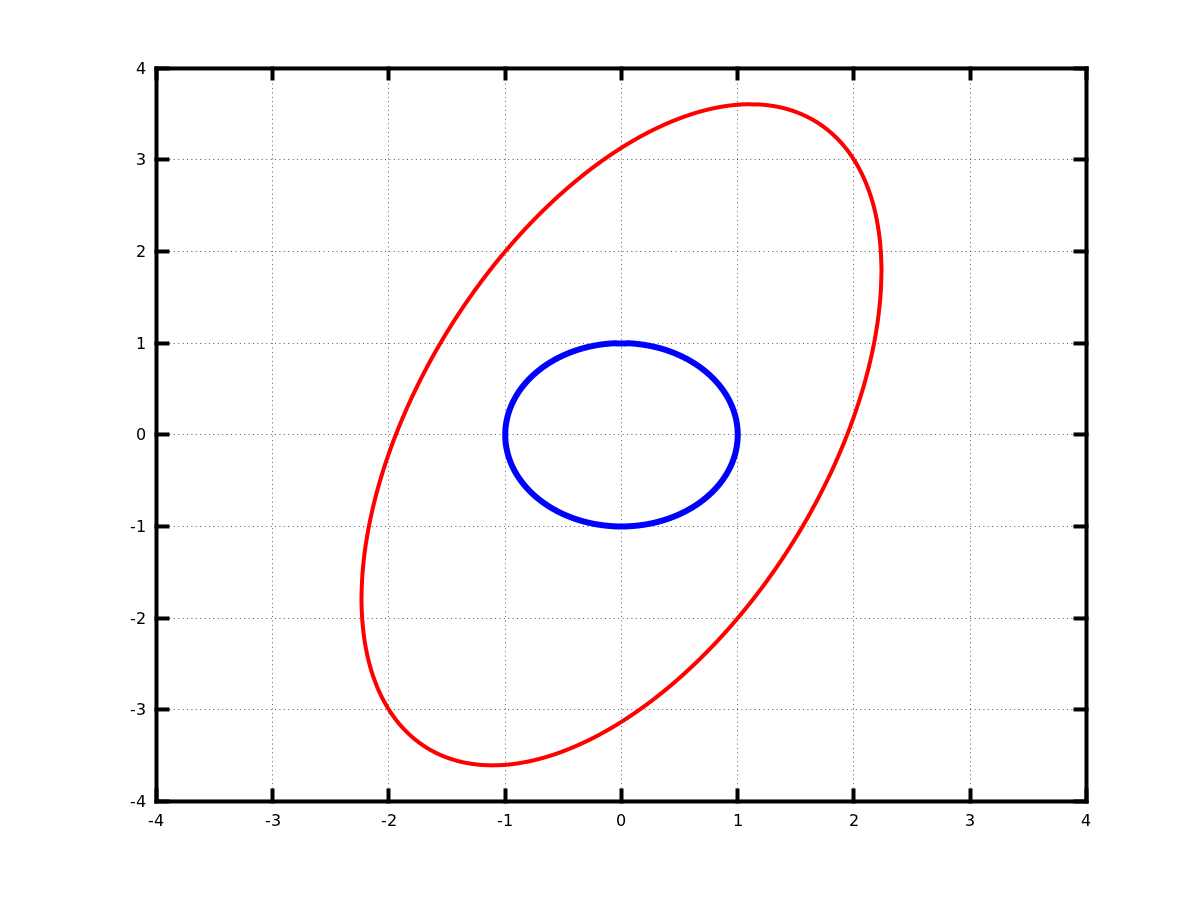
\includegraphics[width=.5\textwidth]{lista11_esfb.png}
        \end{center}

        Agora vamos estudar o caso em que o posto \'{e} incompleto.

        Na figura abaixo encontra-se ilustrado a a\c{c}\~{a}o da matriz $[1 \, 7; \, -7 \, 1]$.
        \begin{center}
            % TODO Refazer figura no Tikz.
            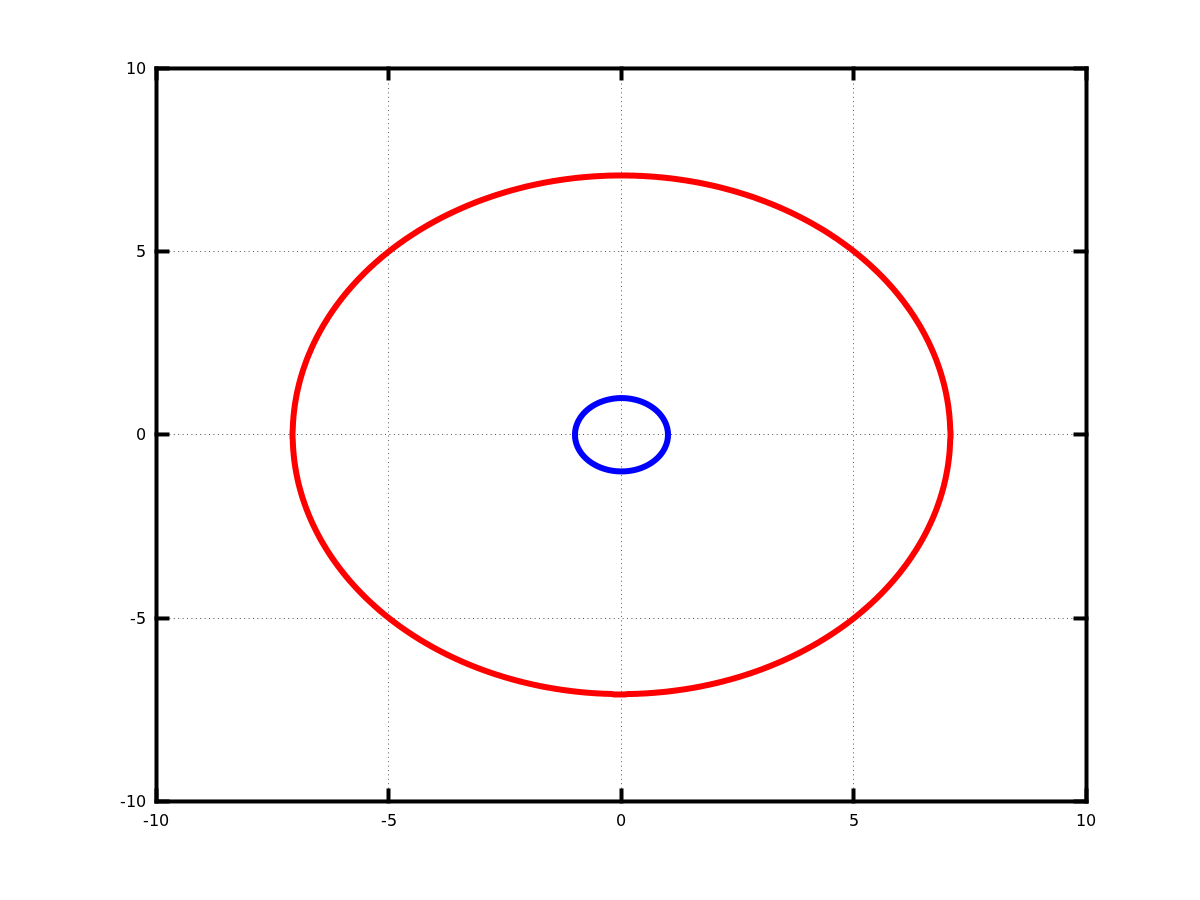
\includegraphics[width=.5\textwidth]{lista11_esfa.png}
        \end{center}
    \end{solution}

    \question Demonstre que a matriz $A$ pode ser representada atrav\'{e}s da decomposi\c{c}\~{a}o SVD reduzida: $A = \hat{U} \hat{D} \hat{V}^t$ e a partir da\'{i} podemos escrever $A = \sum_{i = 1}^r \sigma_i u_i v_i^t$.
    \begin{solution}
        Pela decomposi\c{c}\~{a}o SVD temos que
        \begin{align*}
            A &= \begin{bmatrix}
                u_1 & \ldots & u_r & u_{r + 1} & \ldots & u_m
            \end{bmatrix} \begin{bmatrix}
                \sigma_1 \\
                & \ddots \\
                & & \sigma_r \\
                & & & 0 \\
                & & & & \ddots \\
                & & & & & 0
            \end{bmatrix} \begin{bmatrix}
                v_1^t \\
                \vdots \\
                v_r^t \\
                v_{r + 1}^t \\
                \vdots \\
                v_n^t
            \end{bmatrix} \\
            &= \begin{bmatrix}
                \hat{U} & \tilde{U}
            \end{bmatrix} \begin{bmatrix}
                \hat{D} & \\
                & 0
            \end{bmatrix} \begin{bmatrix}
                \hat{V}^t \\
                \tilde{V}^t
            \end{bmatrix} \\
            &= \begin{bmatrix}
                \hat{U} & \tilde{U}
            \end{bmatrix} \begin{bmatrix}
                \hat{D} \hat{V}^t \\
                0
            \end{bmatrix} \\
            &= \hat{U} \hat{D} \hat{V}^t.
        \end{align*}

        Pela \'{u}ltima express\~{a}o acima verifica-se que $A = \sum_{i = 1}^r \sigma_i u_i v_i^t$.
    \end{solution}

    \question[Equa\c{c}\~{a}o (4.1.8), p\'{a}gina 264, do Watkins\nocite{Watkins:2004:fundamentals}] \'{E} poss\'{i}vel extrair bases para os sub-espa\c{c}os: $\mathcal{I}(A)$, $\mathcal{N}(A^t)$, $\mathcal{I}(A^t)$ e $\mathcal{N}(A)$, a partir dos vetores coluna da matriz $V$ e de $U$. Quais s\~{a}o estas bases? Demonstre estes resultados sem utilizar o Teorema do N\'{u}cleo e Imagem.
    \begin{solution}
        Considerando a decomposi\c{c}\~{a}o SVD, $A = U D V^t$, temos que
        \begin{align*}
            A V &= U D V^t V = U D,
        \end{align*}
        i.e., $A v_i = u_i \sigma_i$, $i = 1, \ldots, r$, e $A v_i = 0$, $i = r + 1, \ldots, n$, e tamb\'{e}m que
        \begin{align*}
            A^t &= V D U^t \Rightarrow A^t U = V D U^t U = V D,
        \end{align*}
        i.e., $A^t u_i = v_i \sigma_i$, $i = 1, \ldots, r$, e $A^t u_i = 0$, $i = r + 1, \ldots, m$.

        Logo,
        \begin{align*}
            \mathcal{I}(A) &= \mathrm{span}\left\{ v_1, \ldots, v_r \right\}, \\
            \mathcal{N}(A) &= \mathrm{span}\left\{ u_{r+1}, \ldots, u_n \right\}, \\
            \mathcal{I}(A) &= \mathrm{span}\left\{ u_1, \ldots, u_r \right\}, \\
            \mathcal{N}(A) &= \mathrm{spam}\left\{ v_{r+1}, \ldots, v_m \right\}.
        \end{align*}
    \end{solution}

    \question[Teorema 4.2.1, p\'{a}gina 266, do Watkins\nocite{Watkins:2004:fundamentals}] Demonstre de duas maneiras diferentes que $\| A \|_2 = \sigma_1 = \sigma_{\max}$.
    \begin{solution}
        Seja $A \in \mathbb{R}^{m \times n}$ e seus valores singulares $\sigma_1 \geq \sigma_2 \geq \ldots \geq 0$. Precisamos mostrar que $\max_{x \neq 0} \| A x \|_2 / \| x \|_2 = \sigma_1$. Primeiro notemos que como $A v_1 = \sigma_1 u_1$ ent\~{a}o
        \begin{align*}
            \frac{\| A v_1 \|_2}{\| v_1 \|_2} = \sigma_1 \frac{\| u_1 \|_2}{\| u_1 \|_2} = \sigma_1.
        \end{align*}
        Logo, $\max_{x \neq 0} \| A x \|_2 / \| x \|_2 \geq \sigma_1$ e agora precisamos mostrar que para nenhum outro vetor induzimos uma norma maior que $\sigma_1$.

        Seja $x \in \mathbb{R}^n$. Ent\~{a}o $x$ pode ser expresso como uma combina\c{c}\~{a}o linear dos vetores singulares a direita de $A$,
        \begin{align*}
            x &= c_1 v_1 + c_2 v_2 + \ldots + c_n v_n.
        \end{align*}
        Como $v_1, \ldots, v_m$ s\~{a}o ortogonormais,
        \begin{align*}
            \| x \|_2^2 &= | c_1 |^2 + | c_2 |^2 + \ldots + | c_n |^2.
        \end{align*}
        Ent\~{a}o
        \begin{align*}
            A x &= c_1 A v_1 + c_2 A v_2 + \ldots + c_r A v_r + c_{r + 1} A v_{r + 1} + \ldots + c_n A v_n \\
            &= \sigma_1 c_1 u_1 + \sigma_2 c_2 u_2 + \ldots \sigma_r + c_r u_r + 0 + \ldots + 0,
        \end{align*}
        onde $r$ \'{e} o posto de $A$. Como $u_1, u_2, \ldots, u_r$ tamb\'{e}m s\~{a}o ortonormais,
        \begin{align*}
            \| A x \|_2^2 &= | \sigma_1 c_1 |^2 + | \sigma_2 c_2 |^2 + \ldots + | \sigma_r c_r |^2 \\
            &\leq | \sigma_1 |^2 | c_1 |^2 + | \sigma_2 |^2 | c_2 |^2 + \ldots + | \sigma_r |^2 | c_r |^2 \\
            &\leq | \sigma_1 |^2 | c_1 |^2 + | \sigma_1 |^2 | c_2 |^2 + \ldots + | \sigma_1 |^2 | c_r |^2 \\
            &\leq | \sigma_1 |^2 \left( | c_1 |^2 + | c_2 |^2 + \ldots + | c_r |^2 \right) \\
            &= \sigma_1^2 \| x \|_2^2.
        \end{align*}
        Logo, como $\| A x \|_2 \geq \sigma_1$ e $\| A x \|_2 \leq \sigma_1$ concluimos que $\| A x \|_2 = \sigma_1$.
    \end{solution}

    \question[Teorema 4.2.4, p\'{a}gina 267, do Watkins\nocite{Watkins:2004:fundamentals}] Se $A : n \times n$, n\~{a}o singular, qual o n\'{u}mero de condi\c{c}\~{a}o de $A$, na norma $2$?
    \begin{solution}
        Sabemos que o n\'{u}mero de condi\c{c}\~{a}o de $A$ na norma $2$, $\kappa_2(A)$, corresponde a
        \begin{align*}
            \kappa_2(A) &= \| A \|_2 \| A^{-1} \|_2.
        \end{align*}
        Sabemos tamb\'{e}m que $\| A \|_2 = \max_i \sigma_i = \sigma_1$.

        Pela decomposi\c{c}\~{a}o SVD temos que $A = U D V^t$ e portanto
        \begin{align*}
            A^{-1} = V D^{-1} U^t.
        \end{align*}
        Logo, $\| A^{-1} \|_2 = \max_i \sigma_i^{-1} = \sigma_n^{-1}$ e assim concluimos que
        \begin{align*}
            \kappa_2(A) &= \sigma_1 \sigma_n^{-1}.
        \end{align*}
    \end{solution}

    \question[Exerc\'{i}cio 4.2.3, p\'{a}gina 266, do Watkins\nocite{Watkins:2004:fundamentals}] Demonstre que $\| A \|_F^2 = \sum_{i = 1}^r \sigma_i^2$.
    \begin{solution}
        Seja $U \in \mathbb{R}^{m \times n}$ uma matrix ortogonal, i.e., $U^t U = I$ e portanto
        \begin{align*}
            \| U x \|^2 = x^t U^t U x = x^t x = \| x \|^2, \forall x \in \mathbb{R}^n.
        \end{align*}

        Ent\~{a}o, pela decomposi\c{c}\~{a}o SVD temos que
        \begin{align*}
            \| A \|_F^2 &= \| U D V^t \|_F^2 \| D \|_F^2 = \sum_{i = 1}^r \sigma_i.
        \end{align*}
    \end{solution}

    \question Usando a decomposi\c{c}\~{a}o SVD demonstre a rela\c{c}\~{a}o e obtenha o menor valor para a constante $\alpha$: $\| A \|_2 \leq \| A \|_F \leq \alpha \| A \|_2$.
    \begin{solution}
        Pelo Teorema 4.2.1 do Watkins\nocite{Watkins:2004:fundamentals} temos que $\| A \|_2 = \sigma_1$ e pelo exerc\'{i}cio anterior temos que $\| A \|_F^2 = \sum_{i = 1}^r \sigma_i^2$. Ent\~{a}o verifica-se que
        \begin{align*}
            \| A \|_2 &= \sigma_1 \leq \left( \sum_{i = 1}^r \sigma_i^2 \right)^{1/2} = \| A \|_F.
        \end{align*}
        No ``pior'' dos casos temos que $\sigma_1 = \sigma_2 = \ldots = \sigma_r$ e portanto
        \begin{align*}
            \| A \|_F &= \left( r \sigma_1^2 \right)^{1/2} = \sqrt{r} \sigma_1,
        \end{align*}
        logo $\| A \|_F \leq \sqrt{r} \| A \|_2$.
    \end{solution}

    \question Demonstre que $\| A \|_2 = \max | y^t A x | / \left( \| x \|_2 \| y \|_2 \right)$, para $x, y \in \mathbb{R}^n$, $\| x \|_2 = 1$ e $\| y \|_2 = 1$. Esta rela\c{c}\~{a}o \'{e} tamb\'{e}m v\'{a}lida se: $\| x \|_2 \leq 1$ e $\| y \|_2 \leq 1$, $x \neq 0$, $y \neq 0$?
    \begin{solution}
        Pela decomposi\c{c}\~{a}o SVD temos que
        \begin{align*}
            \frac{| y^t A x |}{\| x \|_2 \| y \|_2} &= \frac{| y^t A x|}{\| x \|_2 \| y \|_2} \\
            &= \frac{| y^t U D V^t x |}{\| x \|_2 \| y \|_2} \\
            &\leq \frac{\| y^t U \|_2 \| D \|_2 \| V^t x \|_2}{\| x \|_2 \| y \|_y} \\
            &= \frac{\| y \|_2 \| D \|_2 \| x \|_2}{\| x \|_2 \| y \|_2} \\
            &= \| D \|_2 \\
            &= \| A \|_2.
        \end{align*}
        Logo, concluimos que $\| A \|_2 = \max | y^t A x | / \left( \| x \|_2 \| y \|_2 \right)$ \'{e} uma rela\c{c}\~{a}o v\'{a}lida. 
    \end{solution}

    \question Considere $A : n \times n$, n\~{a}o singular. Demonstre que $\min \| A x \|_2 = \sigma_n$, $\forall x \in \mathbb{R}^n$, $\| x \|_2 = 1$. Como generalizar este resultado para $A : m \times n$?
    \begin{solution}
        Pela decomposi\c{c}\~{a}o SVD temos que $A = U \Sigma V^t$ e portanto $A^{-1} = V^{-T} \Sigma^{-1} U^{-1} = V \Sigma^{-1} U^t$. Deste modo, os valores singulares de $A^{-1}$, em ordem crescente, s\~{a}o $\sigma_n^{-1} \geq \sigma_{n - 1}^{-1} \geq \ldots \geq \sigma_1^{-1} > 0$.

        Aplicando o Teorema 4.2.1 do Watkins\nocite{Watkins:2004:fundamentals}, conclui-se que $\| A^{-1} \|_2 = \sigma_n^{-1}$.

        A generaliza\c{c}\~{a}o deste resultado para $A : m \times n$ envolve a defini\c{c}\~{a}o de pseudoinversa.
    \end{solution}

    \question Julgue verdadeiro ou falso: $\| A x \|_2 \leq \| A \|_F \| x \|_2$.
    \begin{solution}
        Pela decomposi\c{c}\~{a}o SVD temos que
        \begin{align*}
            \| A x \|_2^2 &= \| U D V^t x \|_2^2 \\
            &= x^t V D U^t U D V^t x \\
            &= x^t V D D V^t x \\
            &= D D x^t V V^t x \\
            &= D D x^t x \\
            &= x^t D D x \\
            &= \| D x \|_2^2.
        \end{align*}
        Logo, $\| A x \|_2 = \| D x \|_2 \leq \| D \|_2 \| x \|_2 = \| A \|_F \| x \|_2$.
    \end{solution}

    \question Liste os argumentos que podemos usar para afirmar que $\mathrm{posto}(A) = r$.
    \begin{solution}
        % TODO Fazer esse exerc\'{i}cio.
    \end{solution}
\end{questions}
\bibliographystyle{plain}
\bibliography{bibliography}
\end{document}
